% Paper 1 draft, sections 3-6. Working draft 2026-11-23.
% Numbers trace to: docs/gated_monitor_comparison_results.md, docs/gated_monitor_null_calibration_results.md,
% docs/r7_adaptation_strength_sweep_results.md, scripts/g1_kelly_check.py.

\section{Growth-rate prediction}\label{sec:prediction}

\paragraph{Setting.}
A deployed policy $\pi$ and a reference policy $\pi_{\mathrm{ref}}$ act on a stream of events. The paired
decision cost $c_t = \mathrm{cost}(\pi(X_t),Y_t)-\mathrm{cost}(\pi_{\mathrm{ref}}(X_t),Y_t)\in[-5,5]$ is observed only
when a label is bought. Let $A_t=\mathbf 1[\pi(X_t)\neq\pi_{\mathrm{ref}}(X_t)]$ be the disagreement indicator and $\rho=\Pr(A_t=1)$.
Because the cost depends on the prediction and the label only, $c_t=0$ whenever $A_t=0$. The null is
$\mathbb E[c_t\mid\mathcal F_{t-1}]\le\varepsilon$, and the monitor raises an alarm when a betting e-process crosses $1/\alpha$.
Labels cost money; the monitor holds a reserve equal to a fraction $r$ of the cost of labelling every event.

\paragraph{Two query rules.}
\emph{Uniform} labelling queries every event with probability $r$, giving the inverse-propensity increment
$Z_t=-\varepsilon+L_tc_t/r$ with support bound $B_u=5.1(2/r-1)$ (the prediction-powered bound).
\emph{Gated} labelling never queries an agreement, since its cost is known to be zero, and queries a disagreement with
probability $q_t$, giving $Z_t=-\varepsilon+A_tL_tc_t/q_t$ with predictable support bound $B_t=5/q_t+\varepsilon$.
Gating at rate $q_D=\min(1,r\,\bar\tau_{\mathrm{val}}/\overline{A\tau}_{\mathrm{val}})$ spends the same expected label budget
as uniform labelling at rate $r$ ($\tau$ is the label price).

\paragraph{Growth.}
With stake $s$ the e-process multiplies by $1+sZ_t/B_t$, so the per-event growth is
$G(s)=\mathbb E\log(1+sZ_t/B_t)$ and the monitor uses the stake grid $\{0.05,0.1,0.2,0.4,0.8\}$.
For an interior optimum, $G\approx\mu^2/(2\,\mathbb E Z^2)$ with $\mu$ the mean excess cost, so the ratio of growth rates is
the ratio of second moments:
\[
\frac{G_{\mathrm{gated}}}{G_{\mathrm{unif}}}\;\approx\;\frac{\mathbb E Z_u^2}{\mathbb E Z_g^2}\;\approx\;
\frac{\rho\,\mathbb E[c^2\mid A{=}1]/r}{\rho\,\mathbb E[c^2\mid A{=}1]/q_D}=\frac{q_D}{r}.
\]
When $q_D=r/\rho<1$ this is $1/\rho$: the gated monitor pays only for events that carry information.
When the budget covers every disagreement ($q_D=1$) it is $1/r$. In both regimes the ratio is
$\min(1/\rho,1/r)$. This is the $1/\rho$ label saving of paired auditing~\citep{discern}, restated as an evidence-growth ratio at matched spend.

\paragraph{Support bounds enlarge the gain.}
A bounded e-process cannot stake more than $B$ allows: with a stake grid capped at $0.8$ the effective bet per unit of $Z$ is $s/B$.
The uniform arm's bound $B_u=5.1(2/r-1)$ is $9$--$24\times$ larger than the gated arm's across the four budgets, so its stakes are
pinned near the cap. Active inverse-propensity e-processes carry the same range condition, $\lambda\le(1/q_{\min}-\theta)^{-1}$~\citep{xu2024active}.
We compute $G$ exactly, enumerating the query coin, for each arm with its own bound and the registered grid on the realised post-onset
paths of the \texttt{boundary\_local\_harm} scenario (20 seeds per budget). Table~\ref{tab:prediction} gives the result.

\begin{table}[t]
\centering\small
\caption{Gated-to-uniform evidence-growth ratio. ``Small-signal'' is $\min(1/\rho,1/r)$ with $\rho=0.084$;
``uncapped'' maximises the stake continuously; ``registered grid'' uses the monitor's stake grid and each arm's support bound.
The registered prediction was made before any run.}
\label{tab:prediction}
\begin{tabular}{lrrrrr}
\toprule
$r$ & Small-signal & Uncapped & Reg.\ grid & Reg.\ prediction & Measured \\
\midrule
0.02 & 11.9 & 12.4 & 20.0 & 18   & 17.5 \\
0.05 & 11.9 & 12.5 & 19.7 & 18   & 20.6 \\
0.10 & 10.0 & 10.1 & 15.5 & 15   & 14.7 \\
0.20 & 5.0  & 5.1  & 7.6  & 7.5  & 7.2  \\
\bottomrule
\end{tabular}
\end{table}

\begin{figure}[t]
\centering
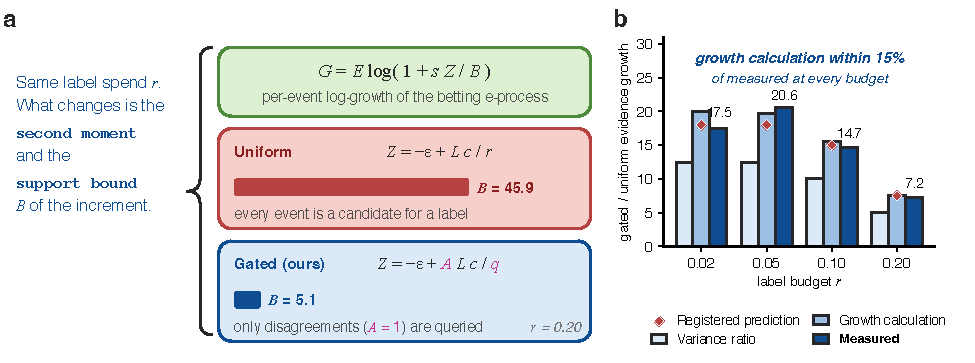
\includegraphics[width=\linewidth]{figures/fig_growth2.pdf}
\caption{The gating gain is predicted within $15\%$ at every label budget. \textbf{a} At the same label spend $r$, gated and uniform labelling differ in the second moment of the increment $Z$ and in its support bound $B$ (bars drawn to scale at $r=0.20$); changed terms are in magenta.
\textbf{b} Gated-to-uniform evidence growth: the variance ratio fixes the order of magnitude, the growth calculation with each arm's bound and the registered stake grid tracks the measured ratio, and the registered prediction (red diamonds) was made before any run.}
\label{fig:growth}
\end{figure}

The variance argument fixes the order of magnitude, and the support bound accounts for the remainder: the registered-grid calculation lands within $15\%$ of the measured ratio at every budget.

\section{Registered protocol}\label{sec:protocol}

\paragraph{Streams.}
Synthetic streams have $n=3200$ events and $d=16$ features. Events $0$--$399$ train the learner, $400$--$799$ are the validation window that seeds pacing and the proxy, and the monitor runs from event $800$.
The deployed classifier uses a fixed $0.5$ threshold; the reference is the cost-minimising rule
(false-negative cost $5$, false-positive cost $1$, tariffs in $[0.5,2.5]$, tolerance $\varepsilon=0.1$, $\alpha=0.05$).
Scenarios are \texttt{stationary} and \texttt{benign\_nuisance} (null controls), \texttt{boundary\_local\_harm}
(an adverse conditional-mean increase localised near the source decision boundary), and \texttt{harmful\_adaptation}
(stationary outcomes, with a policy intervention at event $1600$ that sets actions positive and lifts disagreement from about $8\%$ to $41\%$).

\paragraph{Arms.}
Gated: Horvitz--Thompson at a fixed rate $q_D$ (\texttt{gated\_ht\_fixed}) and at an online-paced rate from a past-only $200$-event tariff window,
clipped to $[0.10,1]$ (\texttt{gated\_ht\_paced}); a proxy-anchored variant; an empirical-Bernstein engine.
Ungated: uniform labelling with a ridge proxy, and the variance-allocated policy.
Published and composed comparators: Timans GRAPA, the prediction-powered e-value (PPE), Xu active betting, SR/CUSUM and a feature-drift sentinel, each given the same gating, correct bounds, label-dollar cap, query coins and proxy access.
Full feedback and a never-alarming monitor are unmatched references.
The reserve is a hard stop: processing ends when the remaining budget falls below the largest label price.

\paragraph{Registration.}
The protocol, the regime map with falsification criteria, the comparator panel and the seed blocks were frozen by hash before the first registered stream.
Calibration used $2{,}000$ streams per null scenario and budget cell with a simultaneous exact $5\%$ bound per arm.
The comparison used $100$ fresh streams per scenario and budget (seeds $58400000$--$58400099$) with two co-primary endpoints:
the post-onset growth ratio at $r=0.20$ (one-sided $97.5\%$ lower bound $\ge2$) and the paired detection difference at $r=0.05$ (lower bound $>0$).
A fidelity stage reproduced the historic uniform-PPI crossings (6/60 at bound 96.9, 47/60 at bound 45.9) exactly before any fresh stream was generated.

\section{Gating results}\label{sec:gating}

\paragraph{Validity.}
In the null cells, the paced gated-HT arm raised between $0$ and $6$ alarms per $2{,}000$ streams, with a largest simultaneous exact upper bound of $0.764\%$.
Every registered arm passed the $5\%$ bound; the largest upper bound anywhere was $1.953\%$ (the PPE source-factor alias, $24/2{,}000$).

\paragraph{Co-primary endpoints.}
Both pass. At $r=0.20$ the paced gated monitor's growth is $7.20\times$ the correctly bounded uniform monitor's (95\% interval $6.88$--$7.55$).
At $r=0.05$ gating wins $100$ discordant streams and loses none (McNemar one-sided $p=7.9\times10^{-31}$).
Table~\ref{tab:r05} lists detection, delay and labels at about equal spend.

\begin{table}[t]
\centering
\caption{\texttt{boundary\_local\_harm}, $r=0.05$, 100 streams.}
\label{tab:r05}
\begin{tabular}{lrrr}
\toprule
Arm & Detection & Censored delay & Labels \\
\midrule
gated HT, paced & 1.00 & 496 & 118 \\
gated HT, paced + Timans GRAPA & 1.00 & 469 & 118 \\
PPE gated & 0.99 & 451 & 118 \\
uniform PPI (bound 45.9) & 0.00 & 1{,}616 & 114 \\
uniform PPI + Timans GRAPA & 0.01 & 1{,}611 & 114 \\
Xu active & 0.00 & 1{,}616 & 115 \\
\bottomrule
\end{tabular}
\end{table}

\paragraph{Registered regimes.}
The regime map predicted that past-paced gating would hold coverage better than a fixed rate when disagreement rises (regime R7). Under \texttt{harmful\_adaptation} fixed gating was equal or better at every budget
($0.86$ against $0.76$ detection at $r=0.10$), and Section~\ref{sec:pacing} follows up this result.

\paragraph{Panel.}
Every gated arm dominates every ungated arm at scarce budgets: at $r\le0.05$ gated arms detect $0.82$--$1.00$ and ungated arms $0.00$--$0.01$.
The strongest selective-label arms are gated HT or PPI with Timans GRAPA and the gated PPE alias (mean detection $0.99$).
When the budget covers all disagreements ($q_D=1$) the regime map predicts, and the results confirm, that every gated variant ties: proxies and allocation rules have nothing left to act on.
The PPI proxy adds nothing over gated HT in \texttt{boundary\_local\_harm} and lowers detection under \texttt{harmful\_adaptation} (mean $0.36$--$0.39$ against $0.50$--$0.59$).

\section{Pacing and the label reserve}\label{sec:pacing}

Under a policy intervention the disagreement rate rises, and the monitor must choose between a fixed gating rate set from validation data and a past-paced rate that lowers $q$ as disagreements arrive.
We vary the intervention strength $s$, the probability that a post-intervention event is forced to the positive action
($s\in\{0.10,0.25,0.50,0.75,1.00\}$; post-onset disagreement $0.12$--$0.41$), across the four budgets with $100$ fresh streams per cell (seeds $61000000$--$61000099$, $2{,}000$ streams in all).

\paragraph{Detection is unchanged by pacing.}
Pooled over the $1{,}900$ harm-path rows, fixed minus paced detection is $+0.005$ (bootstrap $95\%$ interval $-0.006$ to $+0.016$) with the registered betting engine
and $-0.006$ ($-0.018$ to $+0.006$) with Timans GRAPA (Table~\ref{tab:pacing}).

\paragraph{Pacing buys horizon.}
The reserve is a hard stop, so a monitor that spends labels faster than its budget accrues stops earlier.
At full strength and $r=0.05$ the fixed monitor processes $1{,}136$ of $2{,}400$ events and the paced monitor $2{,}111$, at $119$ labels each.
Pacing lowers the post-onset query rate from $0.58$ to $0.14$.
The fixed monitor's horizon shrinks monotonically with $s$ at every budget (at $r=0.02$, $1{,}929\to1{,}131$); the paced monitor's shrinks more slowly.

\paragraph{Pacing lengthens delay.}
A lower $q$ raises the support bound $5/q$, so each label carries less evidence: the range penalty of Section~\ref{sec:prediction} acting on time.
At full strength, censored delay is $598$ (fixed) against $1{,}166$ (paced) events at $r=0.10$, and $401$ against $637$ at $r=0.20$; at $s=0.75$ it is $974$ against $1{,}347$ and $567$ against $783$.
Fixed gating is the faster detector whenever the budget can afford its disagreements; pacing is the choice only when the monitor must keep running past the burst.

\begin{table}[t]
\centering
\caption{Fixed and paced gating at full intervention strength ($s=1.00$), registered betting engine.
Horizon is events processed before the reserve stops the monitor (of 2{,}400). Censored delay is reported for the two budgets where detection is high.}
\label{tab:pacing}
\begin{tabular}{lrrrrrr}
\toprule
 & \multicolumn{2}{c}{Detection} & \multicolumn{2}{c}{Horizon} & \multicolumn{2}{c}{Censored delay} \\
$r$ & fixed & paced & fixed & paced & fixed & paced \\
\midrule
0.02 & 0.06 & 0.04 & 1{,}131 & 1{,}485 & -- & -- \\
0.05 & 0.19 & 0.22 & 1{,}136 & 2{,}111 & -- & -- \\
0.10 & 0.81 & 0.75 & 1{,}220 & 2{,}274 & 598 & 1{,}166 \\
0.20 & 0.99 & 0.99 & 1{,}793 & 2{,}400 & 401 & 637 \\
\bottomrule
\end{tabular}
\end{table}

\begin{figure}[t]
\centering
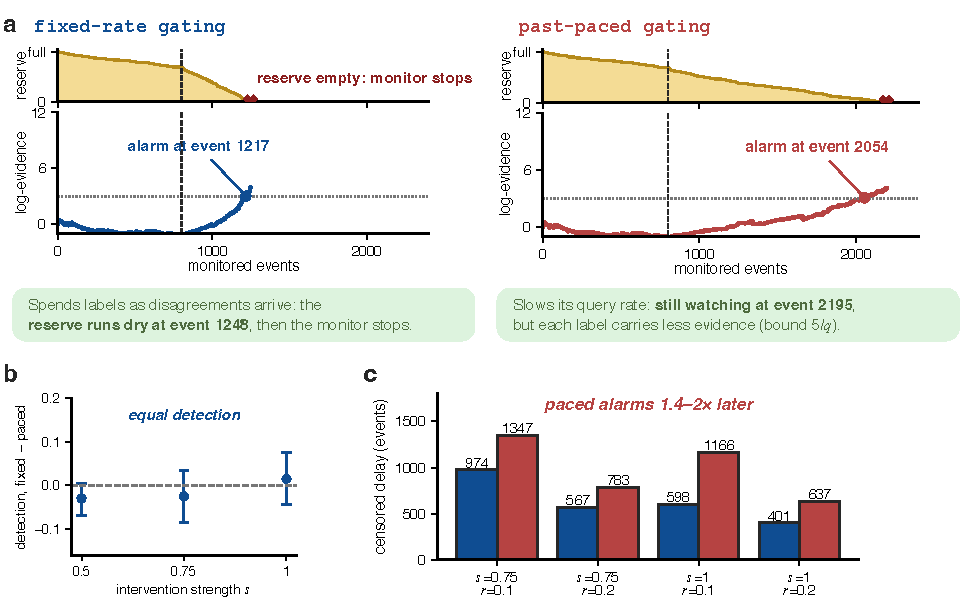
\includegraphics[width=\linewidth]{figures/fig_pacing2.pdf}
\caption{Pacing keeps the monitor alive longer but does not make it detect more often or sooner. \textbf{a} One registered \texttt{harmful\_adaptation} stream ($s=1$, $r=0.10$, seed $61000000$): the fixed-rate monitor's label reserve runs dry at event $1{,}248$ and it alarms at $1{,}217$; the paced monitor is still watching at event $2{,}195$ and alarms at $2{,}054$.
\textbf{b} Pooled over $r\in\{0.05,0.10\}$ and $s\ge0.5$ (100 seeds per cell), fixed minus paced detection has a bootstrap $95\%$ interval containing zero at every strength. \textbf{c} Censored detection delay where both monitors detect.}
\label{fig:pacing}
\end{figure}

\paragraph{A detectability map.}
Full feedback detects from $s=0.50$ ($0.95$). Gated monitors reach $0.87$--$0.99$ at $r=0.20$ for $s\ge0.50$, and $0.56$--$0.86$ at $r=0.10$ for $s\ge0.75$.
At $r\le0.05$ they reach at most $0.29$ at every strength, where uniform labelling detects $0.00$.
Detection rises with both the budget and the intervention strength.
Pre-onset alarm rates stay at or below $1/100$ per cell for every primary arm (exact $95\%$ upper bound $4.7\%$); the PPE alias has one cell at $3/100$.

\begin{figure}[t]
\centering
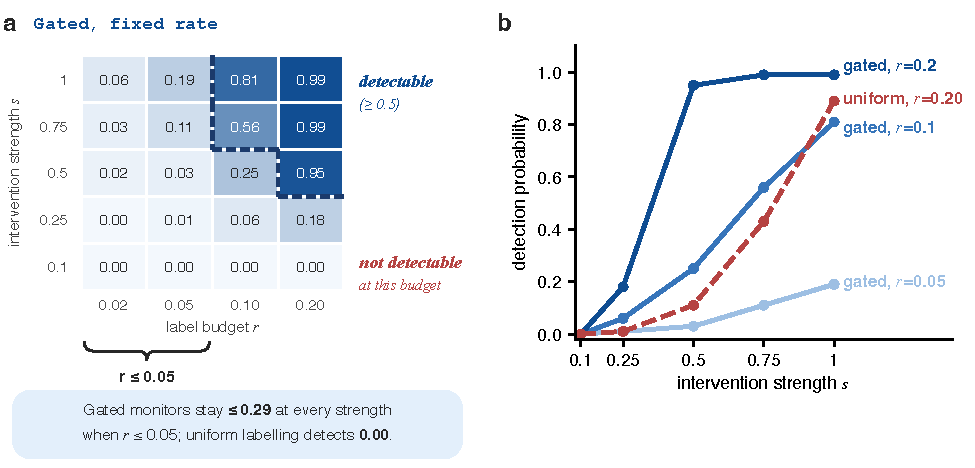
\includegraphics[width=\linewidth]{figures/fig_map2.pdf}
\caption{Gated monitors are detectable once the budget reaches the disagreements the intervention creates. \textbf{a} Detection probability by label budget and intervention strength under \texttt{harmful\_adaptation} (100 streams per cell); the dashed line encloses cells with detection at least $0.5$, and at $r\le0.05$ no strength passes $0.29$. \textbf{b} Detection against strength for three budgets (gated, blue) and for uniform labelling at $r=0.20$ (red, dashed); uniform labelling detects $0.00$ at $r\le0.05$.}
\label{fig:map}
\end{figure}
